\documentclass[tikz,border=12pt]{standalone}
\usepackage[T1]{fontenc}
\usepackage{mathpazo}
\usepackage{amsmath,amssymb}
\usetikzlibrary{arrows.meta, positioning, calc, fit, patterns, decorations.pathreplacing}

\definecolor{stblue}{HTML}{7B97AD}
\definecolor{rwgold}{HTML}{B8995E}
\definecolor{sage}{HTML}{7A9A7E}
\definecolor{dkbrown}{HTML}{3D3530}
\definecolor{wmgray}{HTML}{7B7067}
\definecolor{cream}{HTML}{F9F6F0}
\definecolor{border}{HTML}{D4C9B8}
\definecolor{terracotta}{HTML}{C47A6A}
\definecolor{lavender}{HTML}{907EA0}

\begin{document}
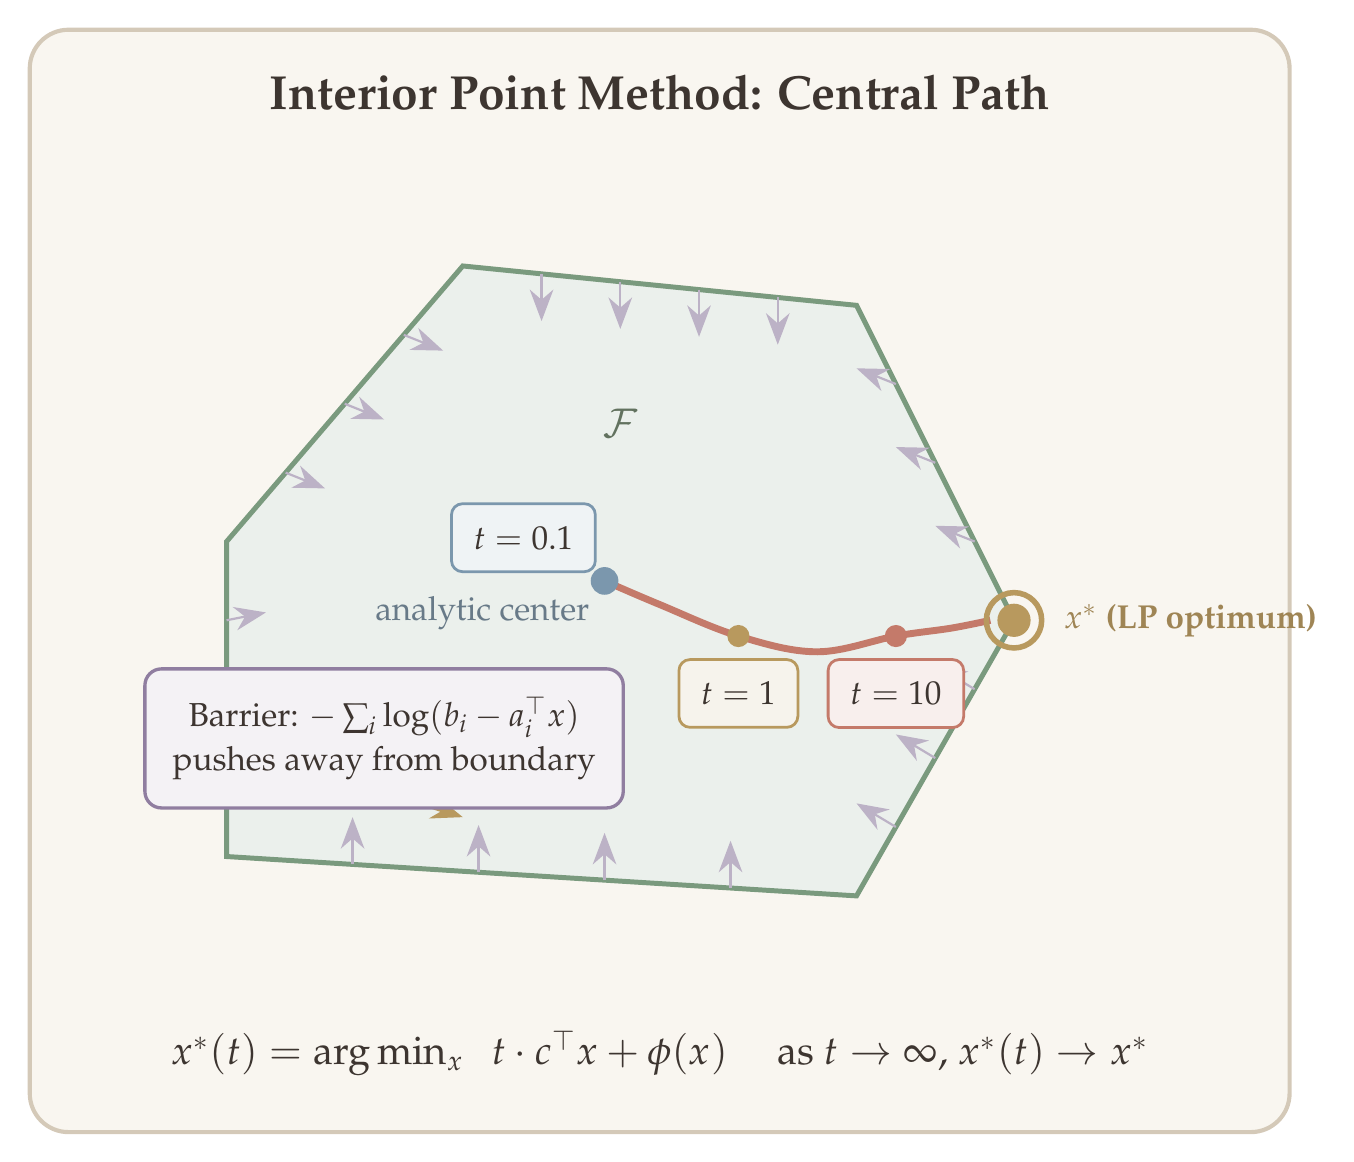
\begin{tikzpicture}[>={Stealth[length=4mm, width=3mm]}, line width=1.5pt]

% Background
\fill[cream, rounded corners=14pt] (-1.5,-2.5) rectangle (14.5,11.5);
\draw[border, line width=1.5pt, rounded corners=14pt] (-1.5,-2.5) rectangle (14.5,11.5);

% Title
\node[font=\LARGE\bfseries, text=dkbrown] at (6.5,10.7) {Interior Point Method: Central Path};

% Feasible region polygon
\coordinate (p1) at (1,1);
\coordinate (p2) at (9,0.5);
\coordinate (p3) at (11,4);
\coordinate (p4) at (9,8);
\coordinate (p5) at (4,8.5);
\coordinate (p6) at (1,5);

\fill[sage!15] (p1) -- (p2) -- (p3) -- (p4) -- (p5) -- (p6) -- cycle;
\draw[sage, line width=1.8pt] (p1) -- (p2) -- (p3) -- (p4) -- (p5) -- (p6) -- cycle;

% Feasible region label
\node[font=\Large, text=sage!60!dkbrown] at (6,6.5) {$\mathcal{F}$};

% Barrier repulsion arrows near each edge (small arrows pointing inward)
% Edge p1-p2 (bottom)
\foreach \t in {0.2, 0.4, 0.6, 0.8} {
  \coordinate (eb) at ($(p1)!\t!(p2)$);
  \draw[->, lavender!60, line width=0.8pt] (eb) -- ($(eb) + (0,0.6)$);
}
% Edge p2-p3 (right-bottom)
\foreach \t in {0.25, 0.5, 0.75} {
  \coordinate (eb) at ($(p2)!\t!(p3)$);
  \draw[->, lavender!60, line width=0.8pt] (eb) -- ($(eb) + (-0.5,0.3)$);
}
% Edge p3-p4 (right-top)
\foreach \t in {0.25, 0.5, 0.75} {
  \coordinate (eb) at ($(p3)!\t!(p4)$);
  \draw[->, lavender!60, line width=0.8pt] (eb) -- ($(eb) + (-0.5,0.2)$);
}
% Edge p4-p5 (top)
\foreach \t in {0.2, 0.4, 0.6, 0.8} {
  \coordinate (eb) at ($(p4)!\t!(p5)$);
  \draw[->, lavender!60, line width=0.8pt] (eb) -- ($(eb) + (0,-0.6)$);
}
% Edge p5-p6 (left-top)
\foreach \t in {0.25, 0.5, 0.75} {
  \coordinate (eb) at ($(p5)!\t!(p6)$);
  \draw[->, lavender!60, line width=0.8pt] (eb) -- ($(eb) + (0.5,-0.2)$);
}
% Edge p6-p1 (left)
\foreach \t in {0.25, 0.5, 0.75} {
  \coordinate (eb) at ($(p6)!\t!(p1)$);
  \draw[->, lavender!60, line width=0.8pt] (eb) -- ($(eb) + (0.5,0.1)$);
}

% Central path (smooth curve from analytic center to optimal vertex)
% Analytic center approximately at centroid
\coordinate (ac) at (5.8,4.5);
% Path curves toward optimal vertex p3
\draw[terracotta, line width=2.5pt, smooth, tension=0.6]
  plot coordinates {(ac) (6.5,4.2) (7.5,3.8) (8.5,3.6) (9.5,3.8) (10.2,3.9) (10.7,4)};

% Points along the path with t labels
\fill[stblue] (ac) circle (5pt);
\node[fill=stblue!12, draw=stblue, rounded corners=4pt, line width=1pt,
      font=\large, text=dkbrown, inner sep=8pt, above left=4pt] at (ac) {$t = 0.1$};
\node[font=\large, text=stblue!70!dkbrown, below left=2pt] at (ac) {analytic center};

\fill[rwgold] (7.5,3.8) circle (4pt);
\node[fill=rwgold!12, draw=rwgold, rounded corners=4pt, line width=1pt,
      font=\large, text=dkbrown, inner sep=8pt, below=8pt] at (7.5,3.8) {$t = 1$};

\fill[terracotta] (9.5,3.8) circle (4pt);
\node[fill=terracotta!12, draw=terracotta, rounded corners=4pt, line width=1pt,
      font=\large, text=dkbrown, inner sep=8pt, below=8pt] at (9.5,3.8) {$t = 10$};

% Optimal vertex
\fill[rwgold] (p3) circle (6pt);
\draw[rwgold, line width=2pt] (p3) circle (10pt);
\node[font=\large\bfseries, text=rwgold!80!dkbrown, right=14pt] at (p3) {$x^*$ (LP optimum)};

% Objective direction
\draw[->, rwgold, line width=1.5pt] (2.5,2) -- (4,1.5);
\node[font=\large, text=rwgold!80!dkbrown, above left] at (2.5,2) {$c$};

% Barrier annotation
\node[fill=lavender!10, draw=lavender, rounded corners=6pt, line width=1.2pt,
      font=\large, text=dkbrown, inner sep=10pt, align=center] at (3,2.5)
  {Barrier: $-\sum_i \log(b_i - a_i^\top x)$\\[2pt]
   pushes away from boundary};

% Bottom formula
\node[font=\Large, text=dkbrown] at (6.5,-1.5)
  {$x^*(t) = \arg\min_x \;\; t \cdot c^\top x + \phi(x)$ \quad as $t \to \infty$, $x^*(t) \to x^*$};

\end{tikzpicture}
\end{document}
